%% 
%% Copyright 2007-2020 Elsevier Ltd
%% 
%% This file is part of the 'Elsarticle Bundle'.
%% ---------------------------------------------
%% 
%% It may be distributed under the conditions of the LaTeX Project Public
%% License, either version 1.2 of this license or (at your option) any
%% later version.  The latest version of this license is in
%%    http://www.latex-project.org/lppl.txt
%% and version 1.2 or later is part of all distributions of LaTeX
%% version 1999/12/01 or later.
%% 
%% The list of all files belonging to the 'Elsarticle Bundle' is
%% given in the file `manifest.txt'.
%% 

%% Template article for Elsevier's document class `elsarticle'
%% with numbered style bibliographic references
%% SP 2008/03/01
%%
%% 
%%
%% $Id: elsarticle-template-num.tex 190 2020-11-23 11:12:32Z rishi $
%%
%%
\documentclass[preprint,12pt]{elsarticle}

%% Use the option review to obtain double line spacing
%% \documentclass[preprint,review,12pt]{elsarticle}

%% Use the options 1p,twocolumn; 3p; 3p,twocolumn; 5p; or 5p,twocolumn
%% for a journal layout:
%% \documentclass[final,1p,times]{elsarticle}
%% \documentclass[final,1p,times,twocolumn]{elsarticle}
%% \documentclass[final,3p,times]{elsarticle}
%% \documentclass[final,3p,times,twocolumn]{elsarticle}
%% \documentclass[final,5p,times]{elsarticle}
%% \documentclass[final,5p,times,twocolumn]{elsarticle}

%% For including figures, graphicx.sty has been loaded in
%% elsarticle.cls. If you prefer to use the old commands
%% please give \usepackage{epsfig}

%% The amssymb package provides various useful mathematical symbols
\usepackage{amssymb}
%% The amsthm package provides extended theorem environments
%%\usepackage{amsthm}

%% The lineno packages adds line numbers. Start line numbering with
%% \begin{linenumbers}, end it with \end{linenumbers}. Or switch it on
%% for the whole article with \linenumbers.
\usepackage{lineno}

%% Русский язык - закомментировать в финальной версии
\usepackage[russian]{babel}

%% advanced mathematics
\usepackage{amsmath}
\usepackage[ruled]{algorithm2e}
\usepackage{multirow}

\usepackage{hyperref}

\journal{Knowledge-Based Systems}

\begin{document}

\begin{frontmatter}

%% Title, authors and addresses

%% use the tnoteref command within \title for footnotes;
%% use the tnotetext command for theassociated footnote;
%% use the fnref command within \author or \address for footnotes;
%% use the fntext command for theassociated footnote;
%% use the corref command within \author for corresponding author footnotes;
%% use the cortext command for theassociated footnote;
%% use the ead command for the email address,
%% and the form \ead[url] for the home page:
%% \title{Title\tnoteref{label1}}
%% \tnotetext[label1]{}
%% \author{Name\corref{cor1}\fnref{label2}}
%% \ead{email address}
%% \ead[url]{home page}
%% \fntext[label2]{}
%% \cortext[cor1]{}
%% \affiliation{organization={},
%%             addressline={},
%%             city={},
%%             postcode={},
%%             state={},
%%             country={}}
%% \fntext[label3]{}

\title{On hyperparameter tuning through Lipschitz global optimization} % and dimensionality reduction}?
%% О настройке гиперпараметров с помощью липшицевой глобальной оптимизации

%% use optional labels to link authors explicitly to addresses:
%% \author[label1,label2]{}
%% \affiliation[label1]{organization={},
%%             addressline={},
%%             city={},
%%             postcode={},
%%             state={},
%%             country={}}
%%
%% \affiliation[label2]{organization={},
%%             addressline={},
%%             city={},
%%             postcode={},
%%             state={},
%%             country={}}

\author[UNN,ITMO]{Konstantin Barkalov}
\author[UNN,ITMO]{Denis Karchkov}
\author[UNN,ITMO]{Evgeny Kozinov}
\author[UNN,ITMO]{Ilya Lebedev}
\author[UNN,ITMO]{Denis Rodionov}
\author[UNN,ITMO]{Marina Usova}

\affiliation[UNN]{organization={Lobachevsky University},%Department and Organization
            addressline={Gagarin Av. 23}, 
            city={Nizhni Novgorod},
            postcode={603022}, 
            %state={},
            country={Russia}}
						
\affiliation[ITMO]{organization={ITMO University},%Department and Organization
            addressline={Lomonosova St. 9}, 
            city={St. Petersburg},
            postcode={191002}, 
            %state={},
            country={Russia}}


\begin{abstract}
%% Text of abstract

The quality of machine learning methods is substantially affected by their hyperparameters, while the evaluation of the quality criterion is a time-consuming operation. Therefore, it is important to develop intelligent methods for selecting optimal values of hyperparameters that require a small number of search trials. In this paper, we propose a new approach to hyperparameter tuning based on the ideas of Lipschitz global optimization. In the framework of this approach, the solution of problems with several parameters is reduced to solving equivalent one-dimensional problems. The reduction is based on the use of space-filling curves (Peano curves). These approaches are implemented in the iOpt open-source framework of intelligent optimization methods.  To demonstrate the advantages of iOpt, we compare it with the well-known Optuna and HyperOpt frameworks when tuning hyperparameters of various machine learning methods on a representative set of datasets. The results show that Lipschitz global optimization methods provide comparable (in terms of quality) results in a significantly shorter time compared to known hyperparameter tuning algorithms.

\end{abstract}

%%Graphical abstract
%\begin{graphicalabstract}
%\includegraphics{grabs}
%\end{graphicalabstract}

%%Research highlights
\begin{highlights}
\item A framework of Lipschitz optimization methods is developed for the tuning of hyperparameters
\item Dimensionality reduction based on Peano space-filling curves is used to solve multidimensional problems
\item A scheme is proposed for reducing the problems, some of whose parameters are categorical, to a single problem with continuous parameters
\item The developed methods (unlike the known methods of hyperparameter tuning) are deterministic, which ensures stable results at different runs of the algorithms 

\end{highlights}

\begin{keyword}
%% keywords here, in the form: keyword \sep keyword
Lipschitz optimization \sep Multiextremal function \sep Hyperparameter tuning

%% PACS codes here, in the form: \PACS code \sep code

%% MSC codes here, in the form: \MSC code \sep code
%% or \MSC[2008] code \sep code (2000 is the default)

\end{keyword}

\end{frontmatter}

\linenumbers

%% main text
\section{Introduction}
\label{sec_intro}

Currently, complex scientific and/or industrial problems are most often solved by numerical methods. Most of such methods, for example, machine learning methods, have hyperparameters, and the choice of specific values of these hyperparameters can determine the efficiency (in a given metric) of the obtained solution under certain constraints on the computation time \cite{Hutter2019,nikitin2021}. The fact that in many cases the difference in the efficiency of the solution obtained with different values of hyperparameters can be quite significant, has resulted in the emergence of the hyperparameter optimization (HPO) problem, as well as the research of approaches to its solution that are implemented in the frameworks for automatic selection of hyperparameters \cite{Tune, optuna, hyperopt,Sherpa}. From the mathematical point of view, the HPO problem corresponds to a global optimization problem with fixed bounds on the variation of hyperparameters.  In certain cases, some of the hyperparameters may be categorical, i.e., they can only assume values from a certain, usually small, number of variants, which necessitates the use of optimization methods capable of solving problems with discrete parameters.

For an end user who wishes to fine-tune the method used by selecting an optimal combination of hyperparameters, the choice of a particular framework is determined by the following factors: 1) efficiency of the methods implemented in the framework that allow solving an HPO problem from the class of problems to which the user's problem belongs; 2) ease of using the  framework from the point of view of description/formulation of the problem of selecting the optimal combination of hyperparameters, organization of the optimum search process, as well as obtaining and analyzing the results. Today, the most common way to organize such an interface is to use the Python programming language, while the frameworks can be written both in this and other languages.

In this paper, we present iOpt \footnote{\url{https://github.com/aimclub/iOpt/}}, a framework of intelligent optimization methods focused on solving problems of selecting optimal values of hyperparameters of various algorithms (including machine learning and heuristic optimization methods). The paper is organized as follows. At the beginning, there is a review of known methods used for hyperparameter tuning. Section \ref{sec_lip} presents the mathematical formulation of the problem, describes approaches to the reduction of multidimensional problems to one-dimensional problems and to the solution of problems with discrete parameters. Section \ref{sec_iOpt} explains the algorithmic basis of global optimization methods implemented in the iOpt framework. In Section \ref{sec_exp}, we present the results of numerical experiments conducted to compare the efficiency of the iOpt framework with other known frameworks on model and applied problems. The conclusion summarizes the findings and plans   for the development of the framework.


\section{Related work}
\label{sec_rel}

The main difficulty in solving the HPO problem is that the search for the optimal combination of hyperparameters requires for each selected variant of their values to solve the corresponding initial problem, for example, the problem of machine learning, and thus can take quite a long time. Thus, any approach to solving the HPO problem will be limited by the number of combinations of hyperparameters that the global optimization method can test before the available computational resource is exhausted.  Certainly, it is difficult in such circumstances to speak about convergence of the method to the global optimum or about any guarantees of finding it. We can only consider the possibility of obtaining an acceptable (from the researcher's point of view) solution. Let us briefly characterize a number of methods that are used to tune hyperparameters (depending on the properties of the initial problem). 

The simplest way to find the global optimum is the exhaustive search method (поиска по равномерной \cite{Bao2006} или случайной \cite{Bergstra2012} сетке). By selecting the number of analyzed variants for each of the hyperparameters, searching all the resulting combinations and choosing the best of them in a given metric, we obtain an estimate of the optimum with a certain accuracy \cite{Nevendra2022}. The exhaustive search method is easy to implement, it has perfect parallelism, but it has a significant drawback (an exponential growth of the number of grid nodes as the number of hyperparameters increases). Thus, exhaustive search can be used as a method for solving HPO problems only in "simple" problems where both the number of hyperparameters (one or two) and the time for solving the initial problem with each selected combination of hyperparameters are small. 

Metaheuristic (genetic and similar) algorithms are an alternative to the exhaustive search when the number of hyperparameters increases \cite{Opara2019}. These algorithms are widely used in the absence of a formula-based description of the model under study (``black-box'' model), which is typical for the considered HPO problems \cite{Zhou2021,Yang2022}. Metaheuristic algorithms only weakly depend on the number of hyperparameters, they use information from previous iterations to perform the current one, but due to the randomness inherent in the methods, they guarantee the finding of the global optimum only in the probabilistic sense.

Another approach to finding the global optimum is Bayesian optimization, which is also used to solve ``black-box'' problems \cite{Frazier2018,Archetti2019}. In fact, Bayesian optimization methods build a stochastic model of the function being optimized. The model is iteratively updated on the basis of the information accumulated in the process of searching for the optimum, making it possible to estimate the most probable position of the global optimum at each iteration. Bayesian optimization methods have significantly higher efficiency compared to the exhaustive search, but they are also affected by the ``curse of dimensionality'', albeit to a lesser extent. 

In well-known hyperparameter tuning frameworks, the Tree-Structured Parzen Estimator (TPE) algorithm is widely used \cite{hyperopt,NIPS2011}. TPE is an iterative algorithm, conceptually close to Bayesian optimization methods. Before the algorithm starts, a search region in the hyperparameter space must be specified and the function to be optimized must be defined. In the course of its work, the method performs trials in the search region and then uses these trials to construct estimates of the distribution of the best and all other results in the hyperparameter space. Next, the combination of hyperparameters that gives the maximum expected improvement is searched for. These hyperparameters are then evaluated on the objective function. The described process is repeated until a specified number of iterations is attained or until the time constraint is reached.  

The good results achieved by Bayesian optimization \cite{Joy2020} and TPE \cite{Watanabe2022a,Watanabe2022b} methods are based on the a priori assumption that the function corresponds to a certain stochastic model, such as a Gaussian process \cite{Rasmussen2005}. However, there are other assumptions about the shape of the function in global optimization that yield remarkable results. 

One of such assumptions about the problem to be solved is the assumption of boundedness of relative changes in the objective function. In this case, the function is said to satisfy the Lipschitz condition, and the problem to be solved is called a Lipschitz global optimization problem. For the class of Lipschitz global optimization problems, a number of efficient algorithms have been developed \cite{Jones2021,Paulavicius2020,Strongin2020,Sergeyev2017,PaulaviciusZilinskas2014}, which surpass many other global optimization methods \cite{Sergeyev2018} and have shown their applicability in a number of applications \cite{Kvasov2008,CANDELIERI2019,Gubaydullin2021}.

The iOpt framework contains an implementation of Lipschitz optimization algorithms, which are an extension of the information-statistical global search algorithm described in detail in \cite{Strongin2000,Sergeyev2013}. In particular, the methods have been adapted to solve problems with partially integer parameters, which are very common in HPO problems. The experimental results presented in Section \ref{sec_exp} show that the iOpt framework is not inferior in HPO problems to well-known frameworks having the same purpose (such as Optuna \cite{optuna} and HyperOpt \cite{hyperopt}). 

\section{Lipschitz optimization} 
\label{sec_lip}

\subsection{Problem statement} 

We will consider the problem of finding the global minimum formulated as follows:
\begin{gather}
	\varphi(y^*) = \min \varphi(y), \; y \in D, \label{f_func} \\
	D = \left\{y \in R^N : a_j \leq y_j \leq b_j , \; 1 \leq j \leq N \right\}. \label{f_D}
\end{gather}

We will also assume that the objective function $\varphi(y)$ satisfies the Lipschitz condition in the search domain $D$, i.e.
\begin{equation} \label{f_lip}
	\left| \varphi(y')-\varphi(y'') \right| \leq L\left\| y' - y''  \right\| , \; y',y'' \in D, \; 0<L<\infty.
\end{equation}
Here $ \left\| \cdot \right\|$ denotes the Euclidean norm, and the constant $L$ is not known a priori and is subject to estimation in the process of solution. 

The function $\varphi(y)$ is assumed to be multiextremal and specified in the form of a ``black box'', i.e., of some algorithm for computing its values. Moreover, it is assumed that each search trial (i.e., computing the value of the function at a point in the admissible region) requires significant computational resources. This problem formulation fully corresponds to the task of tuning the hyperparameters of machine learning methods \cite{Joy2020,Wang2021}.


The Lipschitz condition allows the following geometric interpretation. Suppose that a one-dimensional Lipschitz function $f(x)$ (with the known Lipschitz constant $L$) has been computed at two points $x'$ and $x''$. According to condition (\ref{f_lip}), the following inequalities characterizing the behaviour of the function $f(x)$ on the interval $[x', x'']$  are satisfied:
\begin{gather*}
	f(x) \leq f(x') + L(x-x'), \; x \geq x',\\
	f(x) \geq f(x') - L(x-x'), \; x \geq x',\\
	f(x) \leq f(x') - L(x-x''), \; x \leq x'',\\
	f(x) \geq f(x') + L(x-x''), \; x \leq x''.
\end{gather*}

  By virtue of these inequalities, the values of the function at the points of the interval $[x', x'']$ must lie inside the region bounded by the straight lines passing through the points $(x', f(x'))$ and $(x'', f(x''))$ with slopes $L$ and $-L$ (see Fig. \ref{fig1}).

\begin{figure}
\centering
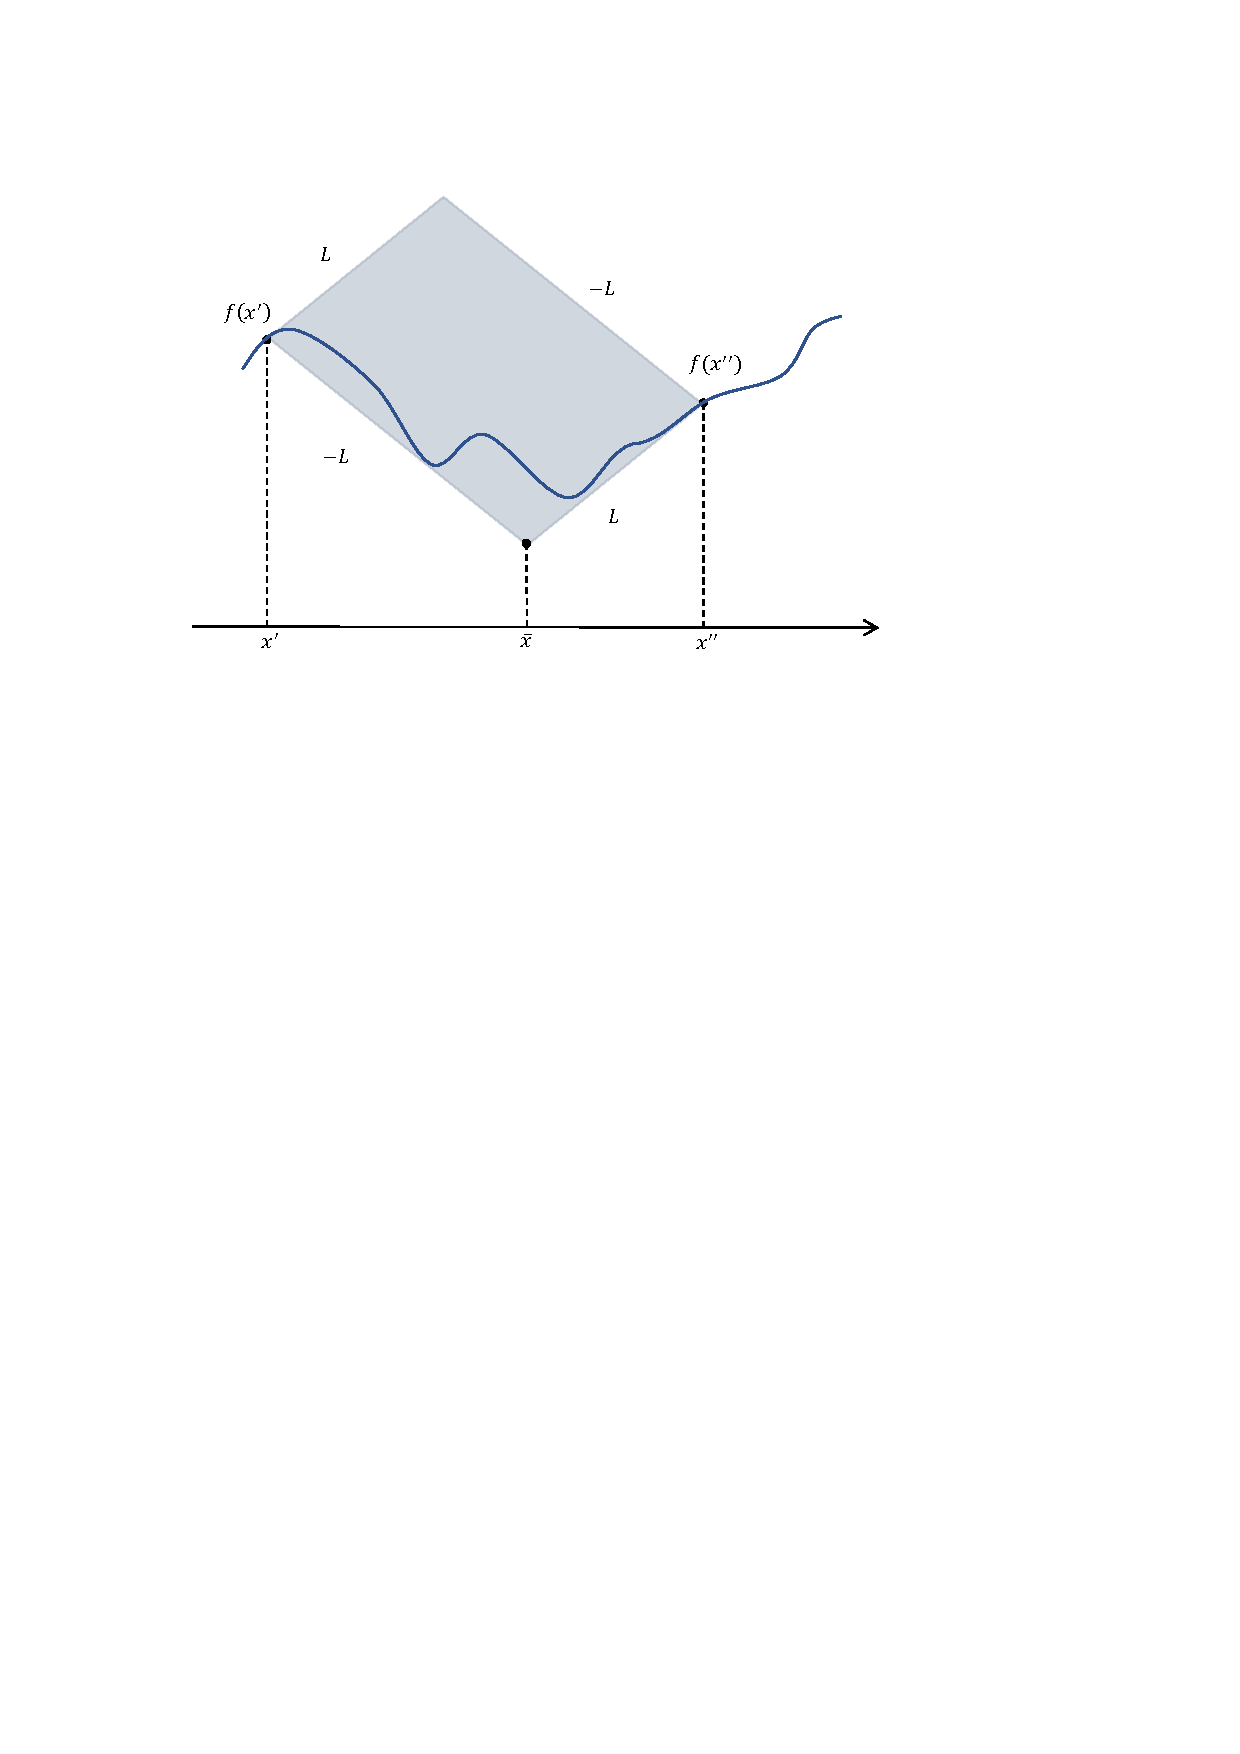
\includegraphics[width=0.8\textwidth]{Fig1.pdf}
\caption{The values of the function $f(x)$ must be inside the area highlighted by colour} \label{fig1}
\end{figure}

Also according to (\ref{f_lip}), we can write the inequality $f(x) \geq F(x)$, where the function  $F(x)$ (called the minorant) is defined according to the formula

\[
F(x) = \max\left\{f(x') - L(x-x'),f(x') + L(x-x'')\right\}, \; x\in [x', x''].
\] 

The smallest value of the minorant $F(x)$ on $[x', x'']$ coincides with the estimate of the smallest value of the function $f(x)$ on this interval. This estimate is reached at the point
\[
\overline{x} = \frac{x'+x''}{2}-\frac{f(x'')-f(x')}{2L}
\] 
and equals
\[
F(\overline{x}) = \frac{f(x')+f(x'')}{2} -L \frac{x''-x'}{2}.
\]

Lipschitz global optimization methods use this idea in their computational rules; the proof of their convergence is also based on this idea (see, e.g.,
\cite{Jones2021,PaulaviciusZilinskas2014,Sergeyev2013,Evtushenko2013}).

\subsection{The problem of dimensionality reduction} 

One of the main difficulties in solving multidimensional global optimization problems is the increase in computational cost as the dimensionality of the problem increases. This difficulty also occurs when solving Lipschitzian global optimization problems. 
For example, solving problem (\ref{f_func}) by means of the uniform grid search with a step $\epsilon$ will require performing
\[
K \approx \prod_{j=1}^N{\frac{b_j-a_j}{\epsilon}}
\]
trials. Obviously, $K$ increases exponentially with increasing $N$. It is possible to reduce the number of trials with the same requirements to the solution accuracy using the adaptive construction of a non-uniform grid in the region of parameter variation. 


A well-known approach to solving the multidimensional problem (\ref{f_func}) is to reduce it to a one-dimensional problem and then apply efficient one-dimensional global optimization algorithms (see \cite{Strongin2000,Sergeyev2013}). A well-proven approach here is to reduce the dimensionality of the problem by means of a Peano-Hilbert curve $y(x), x \in [0, 1]$.  Such a curve uniquely and continuously maps the interval $[0, 1]$ onto the hyperinterval $D$ of (\ref{f_D}), i.e., it fills the entire region $D$.


To solve the Lipschitz global optimization problem, space-filling curves can be applied as follows. If $y(x)$ is a Peano-Hilbert curve, then it follows from the continuity of the objective function $\varphi(y)$ that
\[
\min_{y \in D } \varphi(y) = \min_{x \in [0,1] } \varphi(y(x)),
\]
i.e., the original multidimensional problem (\ref{f_func}) is reduced to a one-dimensional problem.

It is known (see \cite{Strongin2000}) that if a multidimensional function  $\varphi(y), \; y \in D$,  satisfies the Lipschitz condition with the constant $L$, then the reduced one-dimensional function $\varphi(y(x)), \; x \in [0,1]$ satisfies the H{\"o}lder condition
\[
\left|\varphi(y(x'))-\varphi(y(x''))\right|\leq H\left|x'-x''\right|^{1/N}, \; x',x''\in[0,1].
\]
Here, $N$ is the dimensionality of the original problem, and the coefficient
$ H=2 L \sqrt{N+3}$.

Remark 1.  The Lipshitz condition will not be satisfied for the reduced one-dimensional function $\varphi(y(x))$. However, many one-dimensional Lipschitz optimization algorithms can be generalized to the case of H{\"o}lder function minimization. A concrete example of such a generalization is given in subsection \ref{sec_GSA}.

\begin{figure}
\center
\begin{minipage}{0.45\linewidth}
\center{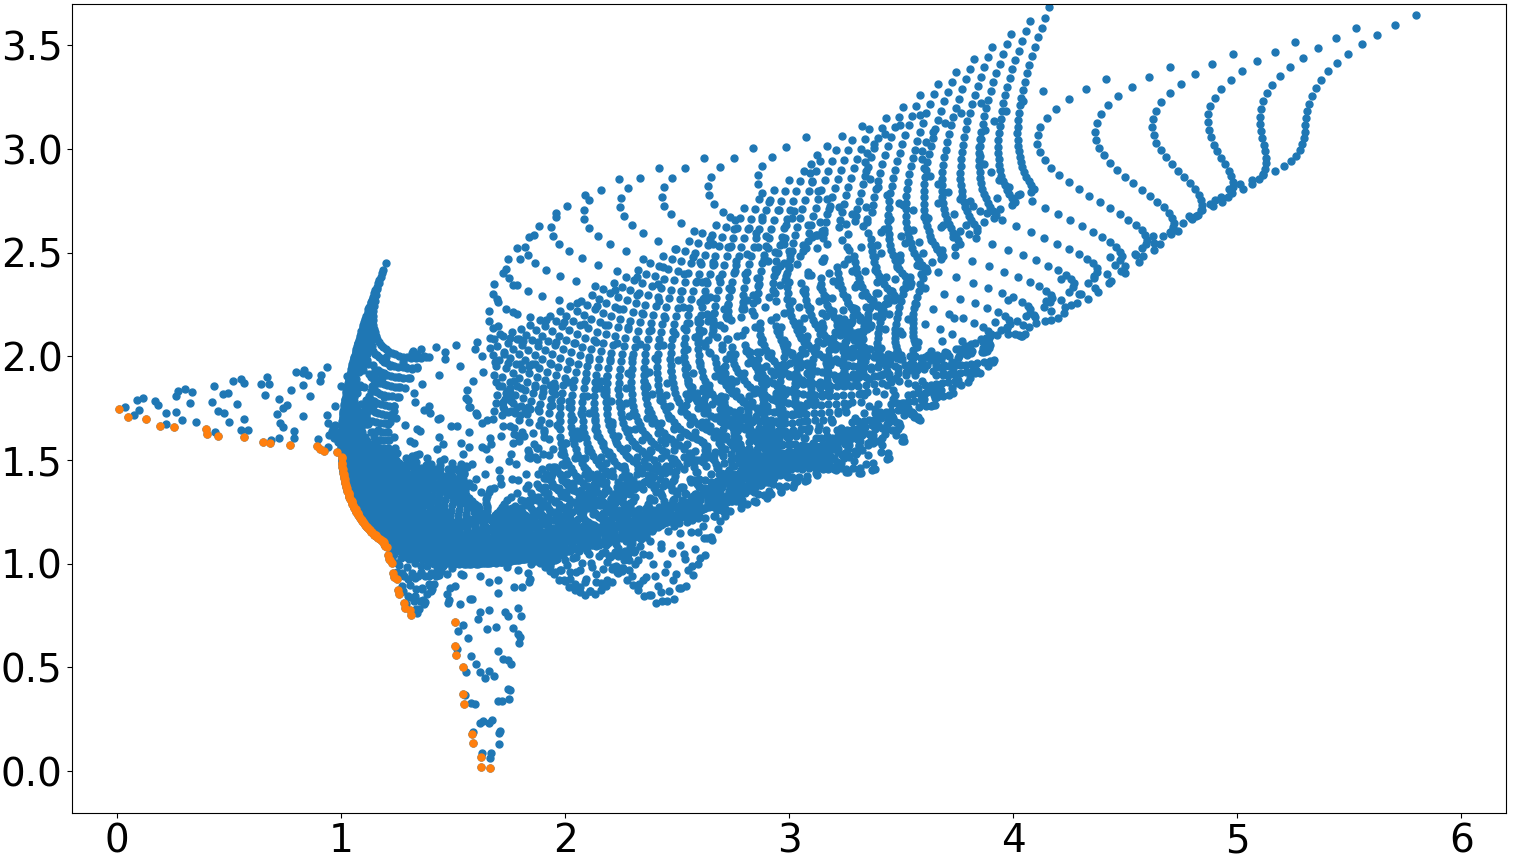
\includegraphics[width=0.9\linewidth]{fig2a.jpg} }
\end{minipage}
\begin{minipage}{0.45\linewidth}
\center{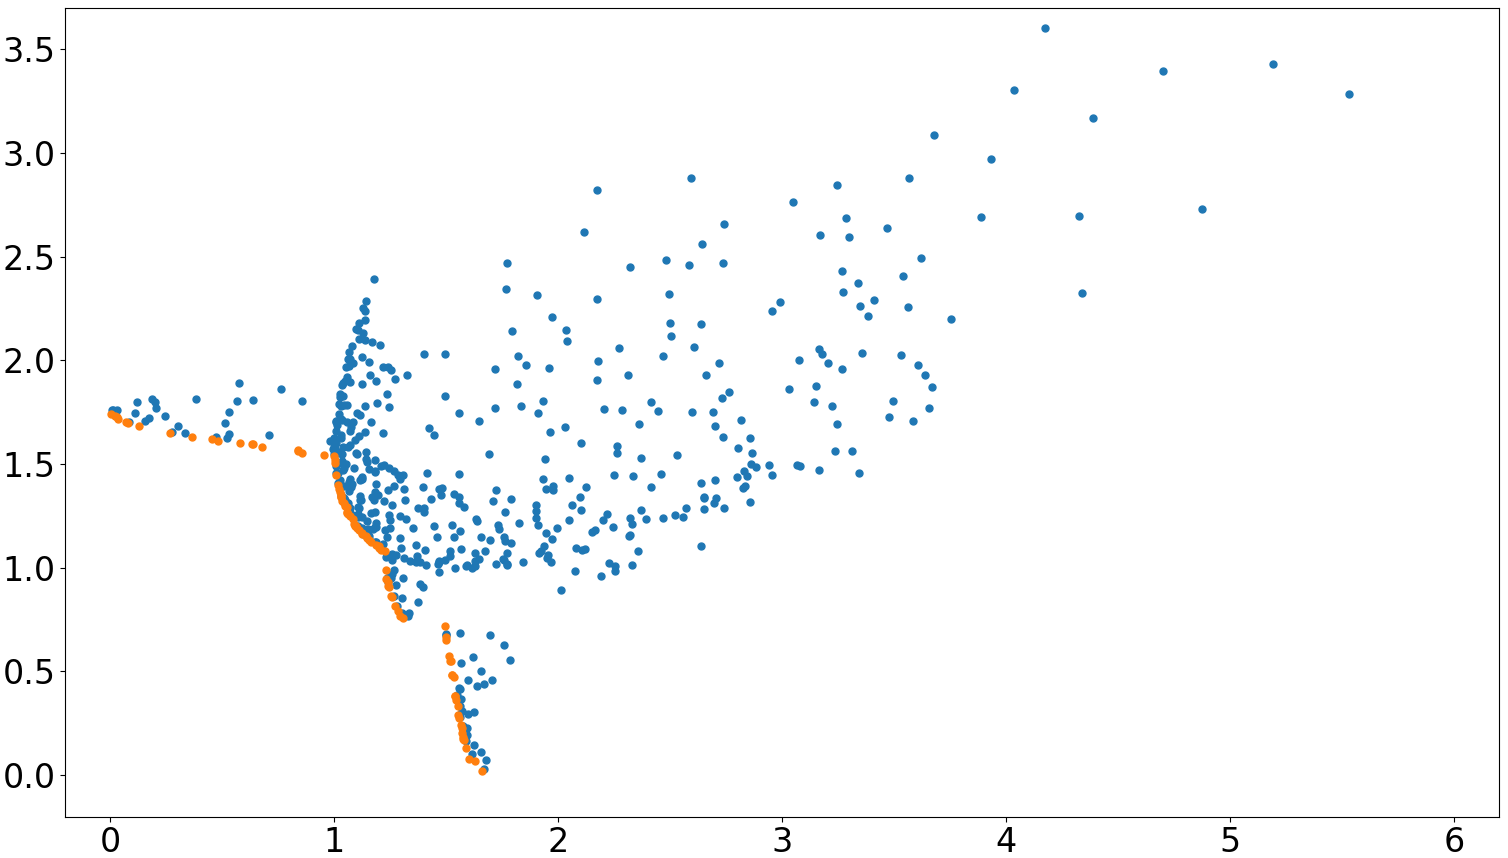
\includegraphics[width=0.9\linewidth]{fig2b.jpg} }
\end{minipage}
\caption{Evolvents $y_m(x)$ with $m=4$.}\label{fig:Peano}
\end{figure}   

Remark 2: The theoretical Peano-Hilbert curve $y(x)$ is defined as a limiting object. Numerical algorithms use evolvents $y_m(x)$, that approximate the true curve with a given density level $2^{-m}$, which depends on the required search accuracy. Efficient schemes for computing several types of evolvents are described in detail in \cite{Sergeyev2013}. For illustration, Fig.~\ref{fig:Peano} shows graphs corresponding to the evolvents $y_m(x)$ with density $m=4$ for dimensions $N=2$ and $N=3$.

\subsection{The problem of discrete parameters}
\label{sec_discr} 

Of particular interest are problems where some of the parameters can assume values from a predetermined finite set, since it is more difficult to construct estimates of the optimum for these problems than for problems with continuous parameters. Many publications address the methods for solving mixed-parameter problems (see, for example, reviews \cite{Burer2012,Boukouvala2016}). Known deterministic methods for solving problems of this class are centered on solving linear or convex problems \cite{Lee2012}. It is suggested that complex multi-extremal problems should be solved using heuristic approaches \cite{Belotti2013}. 

We have proposed and implemented a new deterministic approach to solving problems with mixed parameters; here we give a brief description of it. 
Let the objective function of the problem depend on two parameter vectors: vector $y$, which belongs to the hyperinterval $D$, and vector $u$, which has a finite (and not very large) set of possible values, i.e.
\begin{gather}\label{problem_i}
\min{\left\{ \varphi(y,u) : y\in D \right\}},\\
D=\left\{a_j \leq y_j \leq b_j, \; 1\leq j \leq N \right\}.\nonumber
\end{gather}

Such finite sets of values can characterize many possible combinations of categorical hyperparameters of the machine learning algorithm under study. A typical example is the support vector machine, whose performance is influenced by the continuous regularization parameter $C$ and the kernel coefficient $\gamma$. In this case, the type of kernel function is chosen from a finite set of variants (e.g., polynomial function, radial basis function, sigmoid, etc.). 
%Целочисленные параметры = непрерывные параметры с округлением, добавить комментарий об этом?

Let us number all the different combinations of categorical parameters with integers $s, 1\leq s \leq S$, i.e., let us assign a vector $u_s$ to each number $s$. Then the problem under consideration can be written in the form
\begin{gather}\label{problem_is}
 \min_{s\in\{1,...,S\}}\left[\min{\left\{ \varphi(y,u_s) : y\in D \right\}}\right].
\end{gather}

Using a dimensionality reduction scheme with Peano curves $y(x), x\in [0,1]$,  we can assign to each minimization problem on $y$ a one-dimensional minimization problem
\[
 \min{\left\{ \varphi(y(x),u_s): x \in [0,1] \right\}}, s \in \{1,...,S\}.
\]

Let us now consider the mapping
\[
Y(x)=y(x-E(x)), \; x\in[0,S],
\]
which translates any point of the interval $[0,S]$ to the region $D$ (the notation $E(x)$ corresponds to the integer part of the number $x$) and define the function
\[
f(x) = \varphi(Y(x),u_{E(x)+1}), x\in[0,S],
\]
which has, generally speaking, discontinuities at integer points $x_i = i, 1 \leq i \leq S-1$.
Therefore, the values $z_i = f(x_i)$ at these points will be considered undefined and will not be used in the algorithm.
%, а значения индекса -- равным 0, т.е. $\nu(x_i) = 0$.

Using the introduced notations, we can reformulate the original problem as
\begin{equation}\label{problem_is1}
\min \left\{f(x): x \in [0,S] \right\}.
\end{equation}

Applying the global search algorithm to the solution of problem (\ref{problem_is1}), we will find the solution of problem (\ref{problem_i}). In this case, the main part of trials will be carried out in the $s$-th subproblem, whose solution corresponds to the solution of the original problem (\ref{problem_i}). In the other subproblems, only a small part of trials will be carried out, since the solutions of these subproblems are locally optimal with respect to the solution of the $s$-th subproblem.

\section{iOpt framework} 
\label{sec_iOpt}

The iOpt framework of intelligent optimization methods was developed as part of the ``Strong Artificial Intelligence in Industry'' project. It is designed to select optimal (in a given metric) values of parameters of complex objects and processes, for example, artificial intelligence and machine learning methods. The framework allows fine-tuning of parameters of models and methods used in applied research in various fields of science.  The iOpt framework was designed in the Python programming language using its standard library. To use the framework, you need to have the Pyhon interpreter version 3.8 or higher installed. The framework is open source and is available at \url{https://github.com/aimclub/iOpt}.

The iOpt framework can be used to develop specialized decision support systems for solving the tasks of selecting optimal parameters for complex models or methods. The application area of the framework is focused on the hyperparameter tuning tasks, since this class of tasks involves the problems of multiextremality of the optimization criterion and the lack of a formula-based description of the model under study (a ``black box'' type model).

\subsection{Global search algorithm}
\label{sec_GSA}

The algorithmic core of the iOpt framework is an information-statistical global search algorithm for solving problems of the form (\ref{f_func}), (\ref{f_D}). This algorithm assumes the construction of a sequence of points $y^i$,  at which search trials are performed, i.e., the values of the objective function $z^i = \varphi(y^i)$ are computed. According to the dimensionality reduction scheme used, conducting a trial implies computing $y^i=y(x^i)$, so the result of the trial will be a set of values $(x^i, y^i=y(x^i), z^i = \varphi(y^i))$. 
It is convenient to represent the search information accumulated after conducting $k$ trials as a set in which the corresponding entries are renumbered (by the lower index) in ascending order of $x$, i.e., as a set 
\begin{equation}\label{omega}
\Omega_k = \left\{  (x_i, y_i=y(x_i), z_i = \varphi(y_i)): 1 \leq i \leq k  \right\},	
\end{equation}
where $x_1 < x_2 < ... < x_k$.

The main idea of the global search algorithm is as follows. Let $k \geq 2$ trials be conducted in the search process and the search information $\Omega_k$ from (\ref{omega}) is obtained. To select the point of the next trial for each search interval $(x_{i-1},x_i), 1<i\leq k$, its characteristic is calculated according to the following formula
\begin{equation}\label{R}
R(i) = \Delta_i + \frac{(z_i-z_{i-1})^2}{(r\mu)^2\Delta_i}-2\frac{z_{i-1}+z_i}{r\mu}.	
\end{equation}

Here,  $r>1$ is the algorithm parameter, $\Delta_i=(x_i-x_{i-1})^{1/N}$.  The value $\mu$ is the lower estimate of the H\"older constant of the objective function computed using the search information from (\ref{omega}) by the formula
\begin{equation}\label{mu}
\mu = \max_{1<i\leq k}\frac{\left|z_i-z_{i-1}\right|}{\Delta_i},
\end{equation}
and in case when formula (\ref{mu}) gives the value $\mu=0$, the value $\mu=1$ is used.

A new trial is performed at the point $x^{k+1}$ that belongs to the interval
with the largest characteristic. If the right point of this interval has the number $t$ in the set $\Omega_k$, then the formula for calculating $x^{k+1}$ will look as follows:
\begin{equation}\label{xk1}
x^{k+1} = \frac{x_t+x_{t-1}}{2}- \frac{\mathrm{sign}(z_t-z_{t-1})}{2r} \left(\frac{\left|z_t-z_{t-1}\right|}{\mu}\right)^N.   
\end{equation}

Algorithm \ref{alg_GSA} shows the pseudo code of the Global Search Algorithm. The input data of the algorithm are the objective function $\varphi(y)$ and the search region $D$ from (\ref{f_func}) and (\ref{f_D}), the algorithm parameter $r>1$, the minimum search accuracy $\epsilon > 0$, and the maximum allowable number of trials $K_{max}$. The output parameter of the algorithm is an estimate of the global minimum point $y_{min}$. Additional output parameters can include the value of the function at the minimum point $\varphi(y_{min})$ and the number of trials $k$.

\begin{algorithm}
\LinesNumbered
 \KwIn{$\varphi(y), D, r, \epsilon, K_{max}$}
 \KwOut{$y_{min}$}
 Initialize $k=2$, $\Omega_k= \left\{ (x_1=0, y_1=y(x_1), z_1=\varphi(y_1)), (x_2=1, y_2=y(x_2), z_2=\varphi(y_2)) \right\}$\\
 \While{ $\Delta_t \geq \epsilon$ and  $k \leq K_{max}$}{
  Compute the estimate of the H\"older constant $\mu$ according to (\ref{mu})\\
	\For{$i=1$ \KwTo $k$}{
	Compute the characteristic $R(i)$ according to (\ref{R})\\
	}
	Determine the number $t$, for which $R(t) = \max \left\{ R(i), 1 \leq i \leq k \right\}$
	
	Compute the new trial point $x^{k+1}$ according to (\ref{xk1})
	
	Perform a new trial at the point $x^{k+1}$
	
	Add $(x^{k+1}, y^{k+1}, z^{k+1})$ to the set $\Omega_k$
	
  $k = k + 1$\\
 }
 $l = \arg \min \left\{ z_i, 1 < i \leq k \right\}$\\
 $y_{min} = y_l$, \\ 
 \KwRet{$y_{min}$}
 \caption{Global search algorithm}\label{alg_GSA}
\end{algorithm}

The theory of algorithm convergence as well as some of its modifications are presented in \cite{Strongin2000}.

\subsection{GSA for the problems with categorical parameters}
\label{sec_mGSA}

Let us consider the case when the algorithm to be tuned has both continuous and categorical parameters.  In this case, the categorical parameters can be assigned integer values, and the problem can be reduced to the formulation (\ref{problem_is1}).
Since the solution of problems with partially integer parameters in accordance with the scheme described in Section \ref{sec_discr} implies the solution of problem (\ref{problem_is1}) with a discontinuous objective function, a modification of the algorithm that takes this feature into account is required.

For this purpose, we introduce the classification of points from the search region using a special index $\nu_i=\nu(x_i)$. We will assume the indices of integer points $x_i = i, 0\leq i \leq S$, to be equal to zero, i.e. $\nu(x_i) = 0$. For all other values of $x\in(i,i+1),  0 \leq i < S$, we will assume the index value to be equal to unity, i.e.  $\nu(x) = 1$. Then the result of the trial at some point $x^j\in[0,S]$  will be the set of values $(x^j, \nu^j=\nu(x^j), y^j=y(x^j), z^j = \varphi(y^j))$. In the case of  $\nu^j=0$, the value of $z^j$ will be considered undefined.

The general computational scheme outlined as Algorithm \ref{alg_GSA} will remain the same. The modifications will consist of the following.

1. At the initialization stage, the values $(x^i = i, \nu^i=0, y^i=y(x^i), z^i)$, $ i, 0\leq i \leq S$, i.e., the boundary points of the intervals $(x_{i-1},x_i), 1<i\leq S$, are entered into the set $\Omega_k$ containing the search  information. 
After that, trials are carried out at arbitrary internal points (e.g., midpoints) of the intervals $(x_{i-1},x_i), 1<i\leq S$; the trial results are also added to the search information. Thus, after initialization, the set $\Omega_k$ will contain $k=2S+1$ elements.

2. The computation of the estimate of the H\"older constant $\mu$ according to formula (\ref{mu}) must be performed only for intervals for which $\nu(x_i) = \nu(x_{i-1}) = 1$, i.e., when the values $z_i$ and $z_{i-1}$ are determined.

3. The computation of the characteristic of the search interval $(x_{i-1},x_i), 1<i\leq k$, is performed according to the following rules:
\begin{gather}\label{R_int}
R(i) = \Delta_i + \frac{(z_i-z_{i-1})^2}{(r\mu)^2\Delta_i}-2\frac{z_{i-1}+z_i}{r\mu}, \; \mathrm{if} \; \nu(x_i) = \nu(x_{i-1}) = 1, \nonumber \\ 
R(i) = 2\Delta_i-4\frac{z_i}{r\mu}, \; \mathrm{if} \;  \nu(x_i) = 1, \nu(x_{i-1}) = 0, \nonumber \\ 
R(i) = 2\Delta_i-4\frac{z_{i-1}}{r\mu}, \; \mathrm{if} \;  \nu(x_{i-1}) = 1, \nu(x_{i}) = 0. \nonumber
\end{gather}

Note that the algorithm will not produce intervals whose both boundary points have undefined function values, i.e., $\nu(x_i) = \nu(x_{i-1}) = 0$.

4. The new trial point $x^{k+1}$ will be calculated as follows:
\begin{gather}\label{xk1_int}
x^{k+1} = \frac{x_t+x_{t-1}}{2}- \frac{\mathrm{sign}(z_t-z_{t-1})}{2r} \left(\frac{\left|z_t-z_{t-1}\right|}{\mu}\right)^N, \; \mathrm{if} \; \nu(x_i) = \nu(x_{i-1}) = 1, \nonumber \\    
x^{k+1} = \frac{x_t+x_{t-1}}{2} , \; \mathrm{if} \; \nu(x_i) \neq \nu(x_{i-1}). \nonumber
\end{gather}

Here, $t$ is the number of the search interval that has the maximum characteristic.

We note again that the characteristic $R(i)$ quantifies the possibility of finding a point $x^*$, which is the inverse image of the global optimizer $y^* = y(x^*)$, within the considered interval $(x_{i-1},x_i)$.

\section{Numerical experiments}
\label{sec_exp}

\subsection{Experimental setup}

Datasets

\begin{table}[]
\caption{14 datasets used in the experiments.}
\label{tab:1}
\begin{tabular}{lllllll}
\hline
Name                                                            & Num   & Attributes & Int & Float & Categorical & Classes \\ \hline
Balance                                                         & 625   & 4          & 4   & 0     & 0           & 3       \\
Bank Marketing                                                  & 45211 & 20         & 6   & 4     & 10          & 2       \\
Banknote                                                        & 1372  & 4          & 0   & 4     & 0           & 2       \\
Breast Cancer                                                   & 569   & 9          & 9   & 0     & 0           & 2       \\
CarEvaluation                                                   & 1728  & 6          & 0   & 0     & 6           & 4       \\
CNAE9                                                           & 1080  & 856        & 856 & 0     & 0           & 9       \\
Credit Approval                                                 & 690   & 15         & 0   & 6     & 9           & 2       \\
Digits                                                          & 5620  & 64         & 64  & 0     & 0           & 10      \\
Ecoli                                                           & 336   & 7          & 0   & 7     & 0           & 8       \\
Parkinsons                                                      & 197   & 22         & 0   & 22    & 0           & 2       \\
Semeion                                                         & 1593  & 256        & 256 & 0     & 0           & 10      \\
\begin{tabular}[c]{@{}l@{}}Statlog \\ Segmentation\end{tabular} & 2310  & 19         & 1   & 18    & 0           & 7       \\
Wilt                                                            & 4889  & 5          & 0   & 5     & 0           & 2       \\
Zoo                                                             & 101   & 16         & 16  & 0     & 0           & 7       \\ \hline
\end{tabular}
\end{table}

Metrics


% Please add the following required packages to your document preamble:
% \usepackage{multirow}
\begin{table}[]
\caption{Настраиваемые гиперпараметры для алгоритмов машинного обучения}
\label{tab:2}
\begin{tabular}{llll}
\hline
Метод                    & Параметры            & Тип параметра & Диапазон параметра                                                     \\ \hline
\multirow{7}{*}{XGBoost} & n\_estimators        & Int           & {[}10, 200{]}                                                          \\
                         & max\_depth           & Int           & {[}5, 20{]}                                                            \\
                         & min\_child\_weight   & Int           & {[}1, 10{]}                                                            \\
                         & Gamma                & Float         & {[}0.01, 0.6{]}                                                        \\
                         & Subsample            & Float         & {[}0.05, 0.95{]}                                                       \\
                         & colsample\_bytree    & Float         & {[}0.05, 0.95{]}                                                       \\
                         & learning\_rate       & Float         & {[}0.001, 0.1{]}                                                       \\ \hline
\multirow{3}{*}{\begin{tabular}[c]{@{}l@{}}Support \\ Vector   \\ Classification \\ (SVC)\end{tabular}} &
  Gamma &
  Float &
  {[}$10^{-9}$, $10^{-6}${]} \\
                         & C                    & Int           & {[}$10^1$,$10^{10}${]}                     \\
                         & Kernel               & Categorial    & \begin{tabular}[c]{@{}l@{}}\{‘poly’, ‘rbf’,\\ ‘sigmoid’\}\end{tabular} \\ \hline
\multirow{4}{*}{\begin{tabular}[c]{@{}l@{}}Multi-layer   \\ Perceptron \\ (MLP)\end{tabular}} &
  Activation &
  Categorial &
  \begin{tabular}[c]{@{}l@{}}\{'identity', \\ 'logistic', \\ 'tanh', 'relu'\}\end{tabular} \\
                         & hidden\_layer\_sizes & Int           & {[}2, 30{]}                                                            \\
                         & max\_iter            & Int           & {[}100, 700{]}                                                         \\
                         & Solver               & Categorial    & \begin{tabular}[c]{@{}l@{}}\{'lbfgs', 'sgd', \\ 'adam'\}\end{tabular}  \\ \hline
\end{tabular}
\end{table}

Algorithms for comparison

\subsection{Experimental results}

First result

Second result 

Third result


\begin{table}[]
\caption{Время поиска значений гиперпараметров при однократном запуске алгоритма оптимизации.}
\label{tab:3}
\begin{tabular}{lllllll}
\hline
Dataset &
  \begin{tabular}[c]{@{}l@{}}Optuna \\ random\end{tabular} &
  \begin{tabular}[c]{@{}l@{}}Optuna \\ tpe\end{tabular} &
  \begin{tabular}[c]{@{}l@{}}Optuna \\ cmaes\end{tabular} &
  \begin{tabular}[c]{@{}l@{}}Optuna \\ nsgaii\end{tabular} &
  \begin{tabular}[c]{@{}l@{}}Hyperopt\\ tpe\end{tabular} &
  iOpt \\ \hline
Balance                                                         & 10.8   & 9.2    & 9.0    & 10.6   & 10.3   & \textbf{7.7}    \\
\begin{tabular}[c]{@{}l@{}}Bank \\ Marketing\end{tabular}       & 2888.5 & 3406.5 & \textbf{2704.7} & 3078.6 & 3190.3 & 2963.3 \\
Banknote                                                        & 31.9   & \textbf{12.0}   & 17.7   & 22.1   & 21.7   & 18.4   \\
\begin{tabular}[c]{@{}l@{}}Breast \\ Cancer\end{tabular}        & 9.3    & 7.6    & 6.3    & 8.1    & 8.5    & \textbf{6.0}    \\
CarEvaluation                                                   & 50.9   & 63.3   & 51.0   & 53.1   & 69.5   & \textbf{45.2}   \\
CNAE9                                                           & 295.6  & 207.6  & 318.4  & 262.2  & 253.5  & \textbf{144.9}  \\
\begin{tabular}[c]{@{}l@{}}Credit \\ Approval\end{tabular}      & 14.2   & 12.6   & 13.4   & 13.4   & 15.8   & \textbf{10.8}   \\
Digits                                                          & 132.8  & \textbf{57.5}   & 82.1   & 111.6  & 92.4   & 62.5   \\
Ecoli                                                           & 5.5    & 6.3    & 4.0    & 5.4    & 6.4    & \textbf{3.6}    \\
Parkinsons                                                      & 3.5    & 5.0    & 3.6    & 3.8    & 4.4    & \textbf{2.9}    \\
Semeion                                                         & 218.4  & 119.5  & 157.9  & 135.7  & 193.6  & \textbf{114.2}  \\
\begin{tabular}[c]{@{}l@{}}Statlog \\ Segmentation\end{tabular} & 156.1  & \textbf{55.4}   & 87.1   & 159.2  & 91.6   & 66.5   \\
Wilt                                                            & 70.0   & 75.8   & 68.5   & 67.4   & 78.2   & \textbf{60.9}   \\
Zoo                                                             & 3.0    & 3.9    & 3.0    & 3.1    & 4.2    & \textbf{1.8}    \\ \hline
\end{tabular}
\end{table}


\section*{CRediT authorship contribution statement}

\textbf{Konstantin Barkalov:} Supervision, Conceptualization, Writing - original draft.
\textbf{Denis Karchkov:} Software, Data curation.
\textbf{Evgeny Kozinov:} Methodology, Validation, Writing - original draft.
\textbf{Ilya Lebedev:} Software, Investigation, Writing - original draft.
\textbf{Denis Rodionov:} Software, Investigation.
\textbf{Marina Usova:} Visualization.


\section*{Declaration of competing interest}

The authors declare that they have no known competing financial interests or personal relationships that could have appeared to influence the work reported in this paper.

\section*{Code availability}
%проверить перевод
Software that implements all of the described methods is available in the open repository \url{https://github.com/aimclub/iOpt/}.

\section*{Acknowledgements}
%уточнить ссылку
This research was supported by the research center ``Strong Artificial Intelligence in Industry'' of ITMO University.



%% The Appendices part is started with the command \appendix;
%% appendix sections are then done as normal sections
%% \appendix

%% \section{}
%% \label{}

%% If you have bibdatabase file and want bibtex to generate the
%% bibitems, please use
%%
\bibliographystyle{elsarticle-num} 
\bibliography{bibliography}

%% else use the following coding to input the bibitems directly in the
%% TeX file.

%\begin{thebibliography}{00}

%% \bibitem{label}
%% Text of bibliographic item

%\bibitem{}

%\end{thebibliography}
\end{document}
\endinput
%%
%% End of file `elsarticle-template-num.tex'.
